    % Section 2: SVM
    \section{Support Vector Machines}
        Support Vector Machines (SVM) are a type of supervised machine learning used for classification of data problems. The principles are based on solid and well understood mathematics, making SVM one of the most widely used types of machine learning. SVM has applications in fraud detection, speech and handwriting recognition, and wireless communications \cite{camastra_machine_2008}\cite{zaki_enhanced_2022}.

        The goal of SVM is to create a boundary in a higher dimension space between data points that otherwise would not be linearly separable. Data with $n$ dimensions will be transformed through algorithms known as kernels, into additional dimensions known as feature spaces \cite{noble_what_2006}. For data  $x(t) \in \mathbb{R}^n$ the kernel transform of the data will add an additional dimension where $K_t(x(t)) \in \mathbb{R}^m$ where $m>n$. This is known as the "Kernel Trick" in data science \cite{aizerman_theoretical_1964}.

        Considering two linearly-independent data sets $A$ and $B$ that do not intersect, the data may be passed through a kernel function and transformed into a $n$ dimensional higher space. For each data point, there exists a location on the lower dimensional space, and will now be assigned a new coordinate on the higher dimension space $A(x_1, x_2, ... x_m) \rightarrow K_A(x_1, x_2, ... x_m,... x_n)$ \cite{aizerman_theoretical_1964}.  

        %\begin{figure}[!h] \label{fig:Higher Projection}
                %\centering
                %\includegraphics[scale = 0.3]{Images/Projection to higher space.jpg}
               % \caption{A given two-dimensional data set that is not linearly separable in its original dimension space, is transformed using a Gaussian kernel to create a three-dimensional dataset that is now linearly separable by a plane.}
                %\noindent\makebox[\linewidth]{\rule{0.9\paperwidth}{0.4pt}}
        %\end{figure}

        The data in the feature space projection, may then be linearly separated by a plane where $A$ is above the plane and $B$ lies below. This plane is called a linear hyperplane and is the decision boundary for the data, provided that the optimal kernel has been chosen. Data on one side of the plane belongs to one class, and above to another class \cite{phillips_support_1998}. Hyperplane selection is generated through a supervised training process where regression is used to find the optimal margin between the data points.

        Given $j$ training sets $x$, $(x_1, x_2, ...x_j)$, that exist in the dimension space $n$, the traditional hyperplane function can be given as a simple equation.

        \begin{equation} \label{eq:hyperplane}
            \langle \beta, x\rangle + c = 0
        \end{equation}

        Where $\beta$ is the normal vector to the hyperplane, $\phi \in \mathbb{R}^m$, $c$ is the scalar offset of the hyperplane. The $m$ dimension space is a higher feature space projection of the data within the $n$ dimension space. The solution to the hyperplane can be found by maximizing the distance between the two closest points. This can be done by minimizing the minimum value for the normal vectors, and introducing an error term \cite{elen_adaptive_2022} \cite{burges_tutorial_nodate}. 
        
        \begin{equation}
            \min \frac{|\beta|^2}{2} \kappa(\sum^m_{i=1} \tau_i)
        \end{equation}\

        $\kappa$ is a regularity parameter, and balances the maximization of the distance, and the classification error "slack variable" $\tau$. 
        
        Transformation is highly dependent on the kernel function that is chosen. There are many different kernel functions used for different applications. Kernel combinations are also valid. Transformations may be linear or non-linear in nature. 

        \begin{equation}
            K_t(x,y) = e^{\frac{-(x^2 + y^2)}{2\sigma}}
        \end{equation}
        \begin{equation}
            K_t(x,y) = |x + y|
        \end{equation}
        \begin{equation}
            K_t(x,y) = (xy + 1)^3
        \end{equation}

        The three kernel transformation functions are the RBF, LAbs, and cubic respectively. The LAbs kernel is the only transformation function that is linear, where the others are non-linear transformations. All kernels are functions of two variables being $x$ and $y$, RBF kernel uses an additional hyperparameter $\sigma$ which controls the width of the Gaussian distribution. The larger the value of sigma, the wider the base of the kernel. This has inverse effect on the "tightness" of the data set projection onto the feature space, creating a less-separable data set. 

        Alike many of the other applications, SVM has shown promise in the detection of signals in noise. The use of SVM in signal detection translates the detection problem to a classification problem, i.e. noise vs. signal \cite{tan_detection_2019}. 

        The ability to separate otherwise non-linearly separable data, lends kernel transforms the ability to have discriminatory power against stochastic components in the signal. Given a signal in the presence of noise, the amplitude of the signal will be larger than that of the noise. Thus transformations of the data can artificially enlarge the signals and inflate SNR. This is predicated on the assumption that the noise is mean zero and additive in nature. Discrimination power can be tuned by using different kernel functions. This could be leveraged by signal detection algorithms to increase detection probability in noisy data, particularly in the context of non-white noise. 

        \begin{figure}[t]
            \centering
            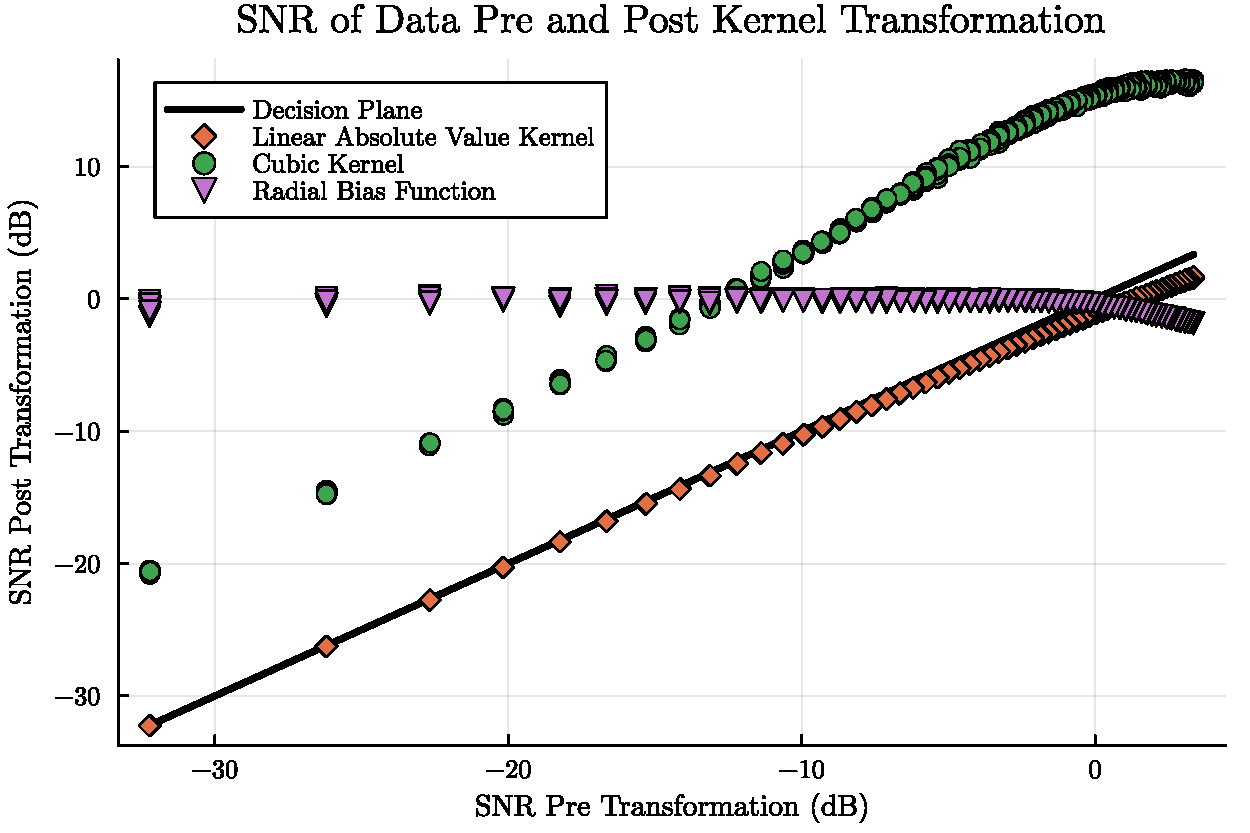
\includegraphics[scale = 0.6]{images/Background/SNRs.pdf}
            \caption{A graphical analysis of the comparison of the original SNR of the data set to the SNR of the data after passed through a kernel transformation function. The three functions examined are the Cubic kernel, Linear Absolute Value kernel, and Radian Bias Function kernel. The black line is the 1 to 1 transformation match, meaning the SNR values are the same before and after transformation. Data that lies above the decision plane is considered to have a positive SNR boost when transformed.}
            \label{fig:SNR_inflation}
        \end{figure}

        \nomenclature{RBF}{Radial Bias Function, synonym for Gaussian kernel}
        \nomenclature{LAbs}{Linear Absolute Value Kernel}
        \nomenclature{$\sigma$}{Gaussian width hyperparameter}
